%%
%% Copy\ref{}right 2022 OXFORD UNIVERSITY PRESS
%%
\documentclass[unnumsec,webpdf,contemporary,medium]{oup-authoring-template}
\makeatletter
  \let\@OrigHeightRecip\relax
  \let\@curXheight\relax
\makeatother
\pdfminorversion=5 % ScholarOne upload compatibility

%--- Preamble --%
% Packages
\usepackage{graphicx}
\usepackage{amsmath}
\usepackage{amssymb}
\usepackage{booktabs}
\usepackage{float}
\usepackage{natbib}
\usepackage{orcidlink} 
\usepackage{subfig}
\usepackage{subcaption}


%--- Journal Meta-data ---%
\journaltitle{Bioinformatics}
\DOI{10.1093/bioinformatics/btzXXX} % TODO: Update with the final DOI from the publisher.
\copyrightyear{2025}
\pubyear{2025}
\access{Advance Access Publication Date: Day Month Year}
\appnotes{Original Paper}
\firstpage{1}

%--- Title and Author ---%
\title[ESMS VAE: Structure-Informed VAE for Protein Engineering]{ESMS VAE: A Structure-Informed Variational Autoencoder for Protein Engineering}
\authormark{Ahn et al.}

% TODO: Replace dummy ORCID iDs with real ones.
\author[1,$\ast$]{Danny Ahn\orcidlink{0009-0006-2820-1498}}
\author[1]{Shihyun Moon\orcidlink{0000-0000-0000-0000}}
\author[1]{Jooyoung Jung\orcidlink{0000-0000-0000-0002}}
\author[1]{Minjae Lee\orcidlink{0009-0002-7484-7338}}

\address[1]{%
 \orgname{Daegu Science High School},
 \street{154 Dongdaegu-ro}, \city{Suseong-gu, Daegu}, \postcode{42111}, \country{Republic of Korea}
}

\corresp[$\ast$]{Corresponding author: \href{mailto:ahnd6474@gmail.com}{ahnd6474@gmail.com}}

% Dummy dates are commented out to prevent compile errors.
%\received{Date}{0}{Year}
%\revised{Date}{0}{Year}
%\accepted{Date}{0}{Year}
\abstract{
Motivation: Protein engineering requires integrating structural insights into sequence generative models. Existing VAEs often ignore inter-residue spatial information, limiting design precision.\\
\Results: We introduce ESMS VAE, which incorporates residue-distance matrices from predicted 3D structures into a CVAE framework. On 162 DMS datasets (sequence length $\leq$512), ESMS VAE achieves a mean Spearman $\rho$ of 0.7779, surpassing Kermut ($\rho$=0.6982) by 11.4\% under supervised settings.\\
Availability and Implementation: Source code, trained models, and datasets are publicly available at \url{https://github.com/Ahnd6474/ESMS-VAE}.\\
Contact: \href{mailto:ahnd6474@gmail.com}{ahnd6474@gmail.com}\\
Supplementary Information: Supplementary data are available online at Bioinformatics.}
\keywords{Variational Autoencoder; Protein Engineering; ESMS; Directed Evolution; Structural Bioinformatics}

\begin{document}
\maketitle
\section{Introduction}\label{sec:introduction}
A Variational Autoencoder (VAE) \cite{kingma2022autoencodingvariationalbayes} is a generative model capable of generating similar but different data from the input. It is usually applied to images and is used to reconstruct and generate images \cite{greener2018protein}. In protein science, VAEs have been suggested to guide the exploration of the vast and empty protein space with their latent space \cite{greener2018protein}. A VAE is made up of an encoder and a decoder. The encoder compresses data and embeds it in a latent space, while the decoder reconstructs the original data from the latent space. The model is trained in a manner that minimizes information loss while compressing data and fits latent space variables to a normal distribution. However, VAEs are susceptible to issues such as posterior collapse, where the decoder ignores the latent space and generates the most common token, and KL vanishing, where an overly perfect fit of the latent space variables to a Gaussian distribution causes a loss of information in the latent space \cite{lucas2019understanding}. Both phenomena are associated with very low KL values, which is why a KL value of around 0.05 is often recommended.

\subsection{Protein VAE}\label{subsec:protein_vae}
It has been demonstrated that the continuous latent space of a VAE can be applied to latent space interpolation and objective-driven amino acid optimization. Early models like Deep-sequence utilized a VAE that takes a Multiple Sequence Alignment (MSA) as input \cite{riesselman2018deepsequence}. It was used to predict mutations, and its latent space could be used as an embedding for other machine-learning tasks. Subsequent protein VAEs continuously evolved by taking a single sequence as input \cite{sinai2017lc}; however, sequences contain smaller information compared to MSAs, and these models usually showed moderate reconstruction rates. A notable advance is ProT-VAE, which uses ProT5 embeddings and a transformer architecture to capture long-distance relations between amino acids \cite{elnaggar2021prottrans}. ProT-VAE showed a nearly 100\% reconstruction rate on fine-tuned protein families.

\subsection{ESM2 and ESMS}\label{subsec:esm}
ESM-2 is a large language model released by Meta AI, trained with masking, and is capable of capturing long and short-distance interactions within a sequence \cite{rives2021biological}. ESM-2 was used as an embedding for ESMFold, a 3D structure prediction model known to have similar capabilities to AlphaFold 2 \cite{lin2022esmfold, jumper2021highly}. It is commonly used as an embedding for various tasks like secondary structure prediction and thermostability prediction. Although its ability to capture structural information is undisputed, it is heavy. Needing a lighter model, Knowledge Distillation \cite{hinton2015distillingknowledgeneuralnetwork} was applied to ESM embeddings. A new small transformer model, ESMS, was trained to mimic ESM2's embedding direction and size. Direction and size were each calculated with cosine similarity and RMSE. Cosine similarity and RMSE on the test set were 0.9647 and 1.2998.

\subsection{Our Contribution}
With ProT-VAE, it has been shown that transformer architectures are capable of capturing hidden information in a sequence. Also, rather than training big transformer models, using a pre-trained model as an embedding was demonstrated to be effective. However, only training with a sequence has clear limits on generalization, function, and versatility. It is clear that structural information must be introduced to train a fully functional VAE. ESMS VAE, in order to overcome such limits, introduced a custom loss function that explicitly forces the VAE to learn and represent structural information in the latent vector space.
A number of additional studies have contributed to advances in generative modeling and protein design \cite{alley2019unified,anand2022protein,anishchenko2021de,baek2021accurate,devlin2019bert,ferruz2022protein,fowler2014deep,frazer2021disease,greener2022guide,higgins2017beta,hopf2017mutation,ingraham2019generative,kuhlman2000native,madani2020progen,meier2021language,notin2022tranception,rao2019evaluating,rao2021msa,repecka2021expanding,russ2020evolution,sohn2015learning,srivastava2014dropout,strokach2020fast,vaswani2017attention,wu2022high,yang2019machine,zuckerkandl1965molecules}.

\section{System and methods}\label{sec:methods}
\subsection{Algorithm}\label{subsec:loss_arch}
To capture structural information, the ESMS model was used to calculate the loss function. ESMS, the student model of ESM2 650M, learned embeddings that capture structural information and were used to calculate the difference in structure between the original (origin) and reconstructed (recon) sequence. This way, the latent vector space was trained to capture structural information. The full ESM2 model could not be used because of limits in computational resources, especially due to memory usage; thus, as a substitute, ESMS was chosen.
ESMS is suitable for this task because it was trained using masking and shows how likely an amino acid is to take place in a certain position. If A and B were both likely to be in a certain position, A and B would have similar embeddings. This is not only because they play a similar role and can be replaced, but also because they both cannot be replaced with certain other amino acids in that position. Thus, structural loss will not penalize amino acids that are likely to be substituted but will penalize those that are not. This also contributes to preventing posterior collapse, which usually occurs by learning the most common amino acid and relying on it. If such an event were to occur, structural loss would penalize it highly and force the VAE to rely on the latent space. This structural loss is similar to perceptual loss in image VAEs. Both concepts try to overcome the information bottleneck from pixel and sequence level matching and try to use deep features that represent perceptual and structural information \cite{johnson2016perceptual}. Image VAE was able to achieve detail preservation: blur reduction, semantic consistency, Robustness against noise, and improved perceptual quality. In ESMS VAE, we can expect conservation of structural information and motifs, robustness against mutation and noise, and improvement in the quality of generated sequences.

The composite loss function is defined as:
\begin{gather}
L = \lambda (L_{\text{MSE}} + L_{\text{COS}}) + \alpha \cdot L_{\text{CE}} + \beta \cdot L_{\text{KL}} \\
\text{where } L_{\text{COS}} = 1 - \text{COS}(\text{ESMS}(\text{origin}), \text{ESMS}(\text{recon})) \nonumber \\
\text{and } L_{\text{MSE}} = \text{MSE}(\text{ESMS}(\text{origin}), \text{ESMS}(\text{recon})) \nonumber
\end{gather}
The weights are set as $\lambda=5$, $\alpha=30$ for epochs $< 100$ (then 0.1), and $\beta=0$ for epochs $< 100$ (then 0.1). These hyperparameters where chosen so that VAE concentrates on reducing CE first and reduces CE even when it is small. $\beta$ Unlike other VAEs is rather unstable, but allows structural and KL loss to have similar losses at beginning of training.

\begin{figure*}[!ht]
\centering
\includegraphics[width=0.8\textwidth]{image_92a7ee.png}
\caption{The architecture of ESMS VAE. An input sequence is processed by a 4-layer Transformer Encoder, which outputs the parameters (mean and log-variance) of the latent distribution. A latent vector is sampled and then reconstructed into the output sequence by a 4-layer Transformer Decoder.}
\label{fig:esms_vae_arch}
\end{figure*}

ESMS VAE is a comparably lightweight transformer with 5.5M parameters, composed of 4-layer transformer encoders and decoders (Figure \ref{fig:esms_vae_arch}). The hyperparameters are detailed in Table \ref{tab:hyperparams}. The Adam \cite{kingma2017adammethodstochasticoptimization} optimizer was used.

\begin{table}[h]
\caption{Hyperparameters for ESMS VAE.}\label{tab:hyperparams}
\centering
\begin{tabular}{@{}ll@{}}
\toprule
\textbf{Parameter} & \textbf{Value} \\
\midrule
Vocab Size & 33 \\
d\_model & 256 \\
Latent Dim & 256 \\
n\_heads & 4 \\
Feed Forward & 512 \\
Dropout & 0.3 \\
\bottomrule
\end{tabular}
\end{table}

\subsection{Implementation and Training}\label{sec:training}
The model was trained using two T4 GPU sessions provided by Kaggle, using a random subsample of the Uni-ref 50 dataset. Monitored learning curves did not show any signs of overfitting (Figure \ref{fig:loss_curves}). The model saved at epoch 500 (VAE\_500) had a final reconstruction rate of 99.976\%. Validation loss values were: Val CE=0.000, COS=0.003, MSE=0.007, and KL=0.002. It exhibited very small latent space values, and the very low KL value suggested potential KL Vanishing (Figure \ref{fig:dist_500}). When noise was added to the latent space, it did not show significant changes in the reconstruction rate. Instead, the model from epoch 380 (VAE\_380) was chosen because it had a KL value closer to the recommended active value of 0.05 and had the lowest validation Cross-Entropy (CE) loss. At epoch 380, the validation losses were: Val CE=0.072, COS=0.010, MSE=0.020, and KL=0.048.

\begin{figure*}[!ht]
\centering
\includegraphics[width=0.8\textwidth]{figure1.png}
\caption{Training and validation loss curves for Cross-Entropy (CE), Cosine Similarity (COS), Mean Squared Error (MSE), and KL Divergence (KL) over 500 epochs. The y-axis is on a log scale.}\label{fig:loss_curves}
\end{figure*}

\begin{figure}[!ht]
    \centering
    \subfloat[mu distribution at epoch 500]{%
        \includegraphics[width=0.48\textwidth]{mu_distribution_500.png}
}
    \hfill
    \subfloat[sigma distribution at epoch 500]{%
        \includegraphics[width=0.48\textwidth]{sigma_distribution_500.png}
}
    \caption{The mean (mu) and standard deviation (sigma) distribution of the latent space at epoch 500, showing signs of KL vanishing.}
    \label{fig:dist_500}
\end{figure}

\begin{figure}[!ht]
    \centering
    \subfloat[mu distribution at epoch 380]{%
        \includegraphics[width=0.48\textwidth]{mu_distribution_380.png}
        }
    \hfill
    \subfloat[sigma distribution at epoch 380]{%
        \includegraphics[width=0.48\textwidth]{sigma_distribution_380.png}
        }
    \caption{The mean (mu) and standard deviation (sigma) distribution of the latent space at epoch 380, showing healthier distributions.}
    \label{fig:dist_380}
\end{figure}

\section{Results}\label{sec:results}
\subsection{Model Reconstruction and Robustness}\label{subsec:reconstruction_robustness}
VAE\_380 achieved a final reconstruction accuracy of 97.17\% on a test set, demonstrating that ESMS VAE generalizes well to different kinds of protein (Figure \ref{fig:dist_380}). To check if the latent space had learned meaningful representations, the following tests were conducted in a teacher-forced manner on completely unseen sequences. VAE\_380's reconstruction rate was tested after adding noise to the latent space. For a test set of about 1000 sequences, the reconstruction rate increased with noise (Table \ref{tab:noise_test}), suggesting the VAE is capable of distinguishing and potentially correcting large noise. This denoising capability was further tested by substituting amino acids with 'X' in a random sample of 100 sequences. The ESMS cosine similarity between the original and reconstructed sequences was 0.9592, which is very close to 1, meaning the VAE is capable of identifying and eliminating noise while not altering structure.

\begin{table}[!ht]
\caption{Reconstruction accuracy under noisy conditions.}\label{tab:noise_test}
\centering
\begin{tabular}{@{}lc@{}}
\toprule
\textbf{Noise Level ($\sigma$)} & \textbf{Mean Reconstruction Accuracy} \\
\midrule
0.1 & 97.77\% \\
1.0 & 98.34\% \\
2.0 & 98.58\% \\
\bottomrule
\end{tabular}
\end{table}

The KL divergence per dimension was checked to ensure the model had not suffered from posterior collapse. The mean KL was 0.04998 with an RMSE of 0.07027. A KL value around 0.05 is considered active, indicating that the latent space is being utilized by the decoder. Random vectors were sampled from the latent space and decoded. These randomly generated sequences were compared with the original sequences and calculated maximum identity; identity mentioned below will mean maximum identity. As shown in Table \ref{tab:novel_generation}, ESMS VAE is not generating copies of the trained sequence but is capable of generating completely different protein sequences.

\begin{table}[!ht]
\caption{Novel generation test results.}\label{tab:novel_generation}
\centering
\begin{tabular}{@{}lc@{}}
\toprule
\textbf{Statistic} & \textbf{Value} \\
\midrule
Median identity & 0.111 \\
90th percentile identity & 0.147\\
Max identity& 0.2121\\
\bottomrule
\end{tabular}
\end{table}

\subsection{Mutation Effect Prediction on DMS dataset}\label{sec:dms}
Model as tested on DMS substitution dataset from protein gym \cite{NEURIPS2023_cac723e5}. Out of all 217 datasets, 162 that had length shorter than 512 were selected. For this, we used a shallow MLP head of seven layers, while using the latent space as an embedding and ran for 300 epochs for each dataset. The result is shown in Figure \ref{fig:dms_result}. Mean of 162 $\rho$(Spearman) value is 0.7779. This result was compared with supervised DMS substitution model, Kermut. Kermut is a model that has first place in the supervised leaderboard. Kermut and simple MLP using ESMS VAE's latent space as features were compared on 162 datasets, and had a mean Spearman constant of 0.6982.

\begin{figure}[!ht]
    \centering
    \includegraphics[width=0.4\linewidth]{ESMS_Kermut.png}
    \caption{Comparison of ESMS VAE and Kermut on Spearman correlation.}
    \label{fig:Spearman_comparison}
    \includegraphics[width=0.5\linewidth]{ESMS_kermut_dist.png}
    \caption{\protect$\rho$ distribution comparison}
    \label{fig:$\rho$ distribution comparison}
\end{figure}

\begin{figure}[!ht]
    \centering
    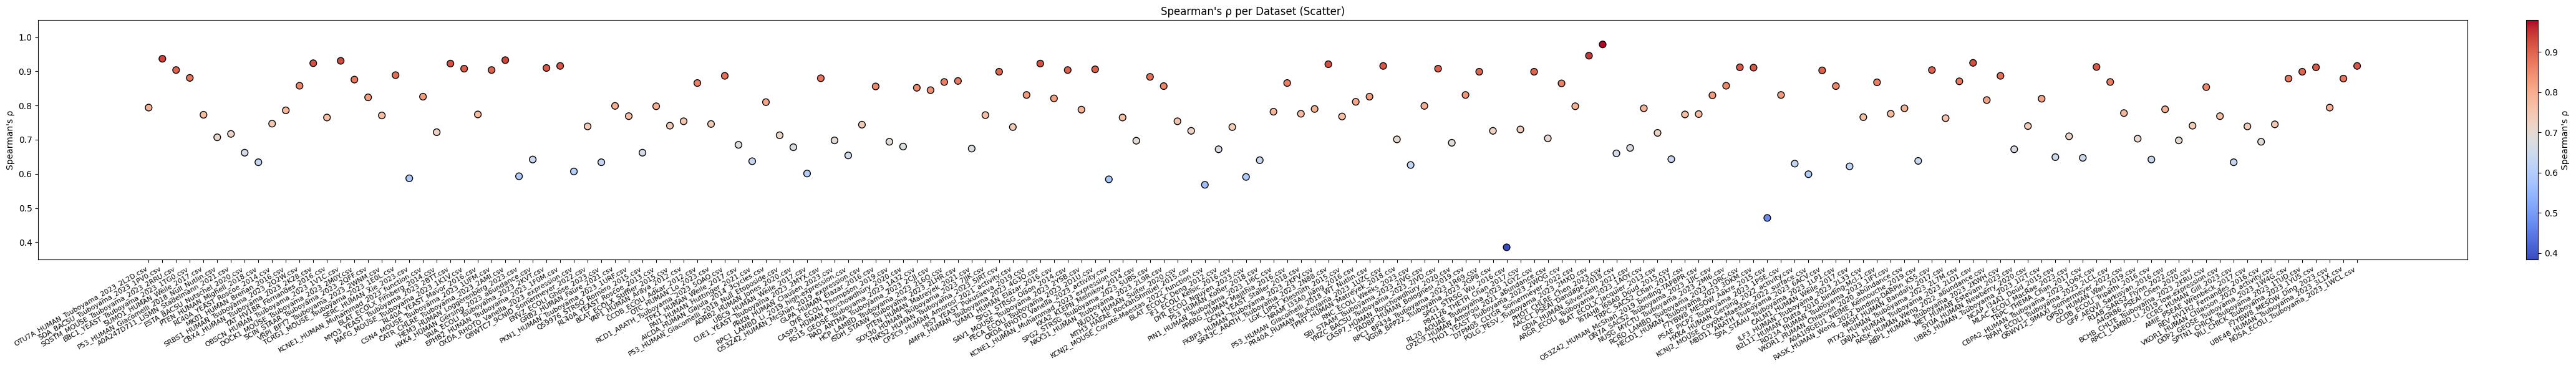
\includegraphics[width=1\linewidth]{DMS.png}
    \caption{Spearman $\rho$ correlation for DMS datasets.}
    \label{fig:dms_result}
\end{figure}
\subsection{Case Study: Fluorescent Protein (FP) Analysis and Generation}\label{sec:fp_application}
The utility of the learned latent space was evaluated on downstream tasks involving Fluorescent Proteins (FPs). FP sequences were collected by hand from FPbase \cite{lambert2022fpbase} and uploaded on kaggle. This was done by hand because there was no suitable API for collection purpose on FPbase. The latent space of the VAE was applied to the classification of FPs and non-FPs, and to estimating maximum absorption and emission wavelengths. A classic Gaussian Process (GP) model was used as the model head \cite{rasmussen2006gaussian}. The GP Classifier (GPC) had a 0.987 5-fold CV accuracy. The GP Regressor (GPR) had an RMSE of 2.70 nm for absorption wavelength (A\_abs) and 3.80 nm for emission wavelength (xem). The classification reports on the train and test sets show the model performs well and is not overfit (Tables \ref{tab:class_report_train} and \ref{tab:class_report_test}).

\begin{table*}[!ht]
\centering
\caption{Classification report on the training set.}\label{tab:class_report_train}
\begin{tabular*}{0.5\textwidth}{@{\extracolsep{\fill}}lrrrr}
\toprule
& \textbf{Precision} & \textbf{Recall} & \textbf{F1-score} & \textbf{Support} \\
\midrule
Non-FP (0) & 0.9920 & 0.9940 & 0.9930 & 501 \\
FP (1) & 0.9880 & 0.9840 & 0.9860 & 250 \\
\midrule
Accuracy & & & 0.9907 & 751 \\
Macro Avg & 0.9900 & 0.9890 & 0.9895 & 751 \\
Weighted Avg & 0.9907 & 0.9907 & 0.9907 & 751 \\
\bottomrule
\end{tabular*}
\end{table*}

\begin{table*}[!ht]
\centering
\caption{Classification report on the test set.}\label{tab:class_report_test}
\begin{tabular*}{0.5\textwidth}{@{\extracolsep{\fill}}lrrrr}
\toprule
& \textbf{Precision} & \textbf{Recall} & \textbf{F1-score} & \textbf{Support} \\
\midrule
Non-FP (0) & 0.9840 & 0.9840 & 0.9840 & 125 \\
FP (1) & 0.9683 & 0.9683 & 0.9683 & 63 \\
\midrule
Accuracy & & & 0.9787 & 188 \\
Macro Avg & 0.9761 & 0.9761 & 0.9761 & 188 \\
Weighted Avg & 0.9787 & 0.9787 & 0.9787 & 188 \\
\bottomrule
\end{tabular*}
\end{table*}

A t-SNE map \cite{maaten2008visualizing} shows that the latent space successfully captures structural information, separating the two classes very well. Non-fluorescent proteins are on the inner side of two curves and fluorescent proteins are on the outside. Visualizations for emission and absorption wavelengths show continuous color gradients, meaning the latent space has separated proteins with different wavelengths and gathered proteins with similar wavelengths together (Figure \ref{fig:tsne}).

\begin{figure}[htbp]
    \centering
    \subfloat[Fluorescence]{%
        \includegraphics[width=0.32\textwidth]{tsne_fluorescence.png}
    }
    \hfill
    \subfloat[Emission Wavelengths]{%
        \includegraphics[width=0.32\textwidth]{tsne_emission.png}
    }
    \hfill
    \subfloat[Absorption Wavelengths]{%
        \includegraphics[width=0.32\textwidth]{tsne_absorption.png}
    }
    \caption{t-SNE visualization of the FP latent space. (a) Clear separation of fluorescent (orange) and non-fluorescent (blue) proteins. (b, c) Continuous gradients for emission and absorption wavelengths, respectively.}
    \label{fig:tsne}
\end{figure}

Collected FP sequences were projected onto the latent space and clustered using K-means. Three clusters were found, with statistics detailed in Table \ref{tab:cluster_stats}. Consensus vectors were calculated based on these clusters and decoded to generate novel sequences. Generated sequences were truncated to the mean length of their cluster since VAEs usually generate meaningless sequences after the original sequence length. These sequences were classified using the trained GPC. As shown in Table \ref{tab:gfp_generation} and Figure \ref{fig:cluster_probs}, Cluster 1 yielded a 100\% success rate. This suggests that the quality and consistency of samples within a cluster are more important than the sheer number of samples for generating new functional proteins. Generated proteins had 96\% ~ 75\% identity with FP sequences that was collected from FPbase. This is likely because the vectors were very alike.

\begin{table}[!ht]
\caption{Statistics for FP clusters identified by K-means.}\label{tab:cluster_stats}
\centering
\begin{tabular}{@{}lrrr@{}}
\toprule
\textbf{Cluster} & \textbf{n (samples)} & \textbf{Mean Length} & \textbf{Std (Length)} \\
\midrule
0 & 22 & 316 & 5.28 \\
1 & 318 & 234 & 10.00 \\
2 & 14 & 118 & 29.71 \\
\bottomrule
\end{tabular}
\end{table}

\begin{table}[!ht]
\caption{Generation of GFP-like sequences from cluster consensus vectors.}\label{tab:gfp_generation}
\centering
\begin{tabular}{@{}lrrr@{}}
\toprule
\textbf{Cluster} & \textbf{Total Generated} & \textbf{Count as GFP} & \textbf{Ratio} \\
\midrule
0 & 4 & 3 & 0.7500 \\
1 & 181 & 181 & 1.0000 \\
2 & 6 & 1 & 0.1667 \\
\bottomrule
\end{tabular}
\end{table}

\begin{figure*}[!ht]
    \centering
    \subfloat[Cluster 0 Probs]{%
        \includegraphics[width=0.3\textwidth]{cluster0_probs.png}
    }
    \hfill
    \subfloat[Cluster 1 Probs]{%
        \includegraphics[width=0.3\textwidth]{cluster1_probs.png}
    }
    \hfill
    \subfloat[Cluster 2 Probs]{%
        \includegraphics[width=0.3\textwidth]{cluster2_probs.png}
    }
    \caption{Probability distribution of generated sequences being classified as GFP for each cluster. Cluster 1 shows high-confidence predictions.}
    \label{fig:cluster_probs}
\end{figure*}

The 3D structures of generated vectors were predicted using the AlphaFold server. For Cluster 1 proteins, iconic beta barrels were found, maintaining a high pLDDT above 90. Proteins from Cluster 0 have two sets containing three beta strands on the inside covered by alpha helices. Proteins from Cluster 2, although not showing a beta-barrel structure, also show structural similarity among themselves, with three beta strands surrounded by alpha helices. This confirms that close vectors in the latent space encode for proteins with similar structures (Figure \ref{fig:structures}).

\begin{figure*}[!ht]
    \centering
    \subfloat[Generated from Cluster 0]{%
        \includegraphics[width=0.30\textwidth]{cluster0_structure.png}
    }
    \hspace{0.03\textwidth}
    \subfloat[Generated from Cluster 1]{%
        \includegraphics[width=0.30\textwidth]{cluster1_structure.png}
    }
    \hspace{0.03\textwidth}
    \subfloat[Generated from Cluster 2]{%
        \includegraphics[width=0.30\textwidth]{cluster2_structure.png}
    }
    \caption{Predicted 3D structures of generated proteins from different clusters show high intra-cluster structural similarity. Cluster 1 notably forms the GFP-like beta barrel.}
    \label{fig:structures}
\end{figure*}


Three sequences were chosen for future in vitro validation based on: 1) GPC prediction, 2) structural likelihood to an original sequence, and 3) whether it needs other fluorescent molecules. Two sequences were chosen from Cluster 1 and one from Cluster 2. The selected sequences are:
\begin{verbatim}
>seq_cluster1_1
MASTPFKFQLKGTINGKSFTVEGEGEGNSHEGSHKGKYVCTSGKLPMSWAALGTS
FGYGMKYYTKYPSGLKNWFHEVMPEGFT
>seq_cluster1_2
MVSTGEELFTGVVPFKFQLKGTINGKSFTVEGEGEGNSHEGSHKGKYVCTSGKLP
MSWAALGTSFGYGMKYYTKYPSGLKNWFF
>seq_cluster2_1
MPRISDKLMKTRWRGFHSIPSIPPDLGGIYGIGEKTSRRKTTEHLYTGRAKDIKS
RLMKHKYGHQAIDRKIRSNIKQKKLSDLRFKFVE
\end{verbatim}

\subsection{Ablation Study}\label{subsec:Ablation_study}
An ablation study as done in this case loss function is ${L=\alpha CE+\beta KL}$ The weights are set as $\alpha =30, \beta=0 $ for epochs $\leq 30 $ else $\alpha=0.1, \beta=0.1$. In the ablation study KL vanishing occurred right after epoch 100 proving role of structural loss in training.

\begin{figure*}[!ht]
    \centering
    \subfloat[CE over epoch]{%
        \includegraphics[width=0.45\textwidth]{CE_blank.png}
    }
    \hfill
    \subfloat[KL over epoch]{%
        \includegraphics[width=0.45\textwidth]{KL_blank.png}
    }
    \caption{CE and KL value over epochs for the ablation study model without structural loss.}
    \label{fig:CE_and_KL_over_epochs}
\end{figure*}

\section{Limitation: Thermo stability (Tm) Prediction}\label{sec:Tm_prediction}
ESMS VAE was used as an embedding, and an MLP head was used to predict Tm value of proteins from multiple classes. As shown in Figure \ref{fig:tm_prediction}a, the MLP did not perform better than just returning the mean value of Tm. This is because none of the 256 latent vectors had a strong correlation with Tm, as seen in Figure \ref{fig:tm_prediction}b. This is likely because ESMS VAE was trained to learn structural likeness rather than the thermo stability of proteins, which explains why the model excelled on the DMS dataset.

\begin{figure*}[!ht]
    \centering
    \subfloat[Tm prediction]{%
        \includegraphics[width=0.48\textwidth]{Tm_pred.png}
    }
    \hfill
    \subfloat[Correlation histogram]{%
    \includegraphics[width=0.48\textwidth]{corre_hist.png}
    }
    \caption{(a) Tm prediction results using an MLP head, showing performance similar to a mean-prediction baseline. (b) A histogram of the correlation coefficients between latent space dimensions and Tm values, indicating no strong correlators.}
    \label{fig:tm_prediction}
\end{figure*}

\section{Discussion}\label{sec:discussion}
ESMS embedding seems to concentrate on structural integrity and likelihood. Thus, the latent space contained structural information and had high Spearman scores in the DMS dataset; however, it seems to have missed Tm-related information. It can be thought of using the AlphaFold structure and contact map as a structural loss; however, AlphaFold commonly takes about 10 to 20 minutes per sequence, which is too long to be applied to mass data. On the other hand the contact map is too costly, using sequences that have a known structure limits the data pool, and the contact map itself requires large memory. It may be suggested that using other PLMs, like ProTrans 5 and ProtBert. Like ESMS and ESM2, it is highly recommended to use smaller versions of PLM.

The latent space contains structural information; thus, like protein space itself, most of the latent space would hold functionless protein. The latent space of ESMS VAE is still too vast, and functional proteins are too scarce. It is highly recommended to use a regressor and a classifier together. The regressor is used to predict your objective, and the classifier will identify a functional protein. So, the regressor will guide your search while the classifier limits your search. This combination will be critical for efficiently navigating the latent space to engineer novel proteins.

\section{Conclusion}\label{sec:conclusion}
ESMS VAE is the first attempt to include structural information in the latent space of a protein VAE using perceptual loss. This concept of structural loss was valid and was capable of creating a latent space that contained structural information.

\section*{Acknowledgements}
ChatGPT (OpenAI), Gemini(Google) was used to assist with language editing and code documentation. All content was authored and verified by the authors in accordance with ISCB’s acceptable use policy.

\section*{Funding}
This work was supported by the Daegu Science High School.

\section*{Author Contributions}

\textbf{Danny Ahn} [lead]: Conceptualization, Methodology, Investigation, Writing – Original Draft, Project Administration.\\
\textbf{Shihyun Moon} [supporting]: Data Curation, Formal Analysis, Visualization.\\
\textbf{Jooyoung Jung} [supporting]: Validation, Writing – Review \& Editing.\\
\textbf{Minjae Lee} [supporting]: Resources, Supervision, Funding Acquisition.


\section*{Data Availability Statement}
The data underlying this article are available in FPbase at \href{https://www.fpbase.org/}{https://www.fpbase.org/} and were uploaded to Kaggle at \href{https://www.kaggle.com/datasets/dannyahn/fluorescent-protein-dataset}{https://www.kaggle.com/datasets/dannyahn/fluorescent-protein-dataset}. The source code and trained models are publicly available on GitHub at \href{https://github.com/Ahnd6474/ESMS-VAE}{https://github.com/Ahnd6474/ESMS-VAE}.

\section*{Conflict of Interest}
The authors declare no conflicts of interest.

\bibliographystyle{natbib} % Corrected bibliography style
\bibliography{reference}

\end{document}